\documentclass[12pt,a4paper]{ctexart}
\usepackage{graphicx}
\usepackage{wrapfig}
\usepackage{float}
\usepackage{siunitx}
\usepackage{subfigure}
\usepackage{caption}
\usepackage{natbib}
\usepackage{listings} % 引入listings宏包用于插入代码
\usepackage{xcolor} % 引入xcolor宏包以支持更多的颜色设置

% 设置Verilog代码样式
\lstdefinestyle{verilog}{
    language=Verilog, % 设置语言为Verilog
    basicstyle=\small\ttfamily, % 设置基本字体样式
    keywordstyle=\color{blue}, % 关键字颜色设置
    commentstyle=\color{gray}\ttfamily, % 注释颜色和样式设置
    stringstyle=\color{red!60!black},
    numbers=left, % 行号在左边显示
    numberstyle=\tiny,
    frame=single, % 添加单线框
    rulecolor=\color{black!30}, % 边框颜色
    breaklines=true, % 允许自动换行
}

\title{实验 4:完整单周期 CPU}
\author{张子康 \ PB22020660}
\date{2024年04月22日}

\begin{document}
\maketitle
\newpage
\section{实验目的与内容}
\subsection{实验目的}
在本次实验中,我们将进一步完善上一次实验设计的 CPU,为其增加分支指令和访存指令的相关功能。
\subsection{实验内容}
\subsubsection{任务 1:访存控制单元设计}
设计访存控制单元 SL\underline{~}UNIT,以正确处理访存指令。
\subsubsection{任务 2:搭建 CPU}
正确实现 CPU 的各个功能模块,并根据数据通路将其正确连接。理论上,你只需要完成 CPU 模块及其子模块的设计,而无需修改其他模块的内容。最终,你需要在 FPGAOL 上上板运行,并通过我们给出的测试程序。
\subsubsection{任务 3:斐波那契数列}
将 Lab1 中编写的斐波那契数列程序(普通版本、大整数版本均可)导出为 COE 文件,在自己设计的 CPU 上运行。相关数据的输入、输出方式不限。
\section{逻辑设计}
\subsection{任务 1:访存控制单元设计}
访存单元代码如下:
\begin{lstlisting}[style=verilog]
//定义访存类型
`define LW 4'b0000
`define LH 4'b0001
`define LB 4'b0010
`define LHU 4'b0011
`define LBU 4'b0100
`define SW 4'b0101
`define SH 4'b0110
`define SB 4'b0111
module SLU (input [31 : 0] addr,
            input [3 : 0] dmem_access,
            input [31 : 0] rd_in,
            input [31 : 0] wd_in,
            output reg [31 : 0] rd_out,
            output reg [31 : 0] wd_out);
// addr_用于存储访存的地址
wire [31:0] addr_;

// 初始化
initial begin
    rd_out=0;
    wd_out=0;
end

// 将计算出的访存地址存储在addr_中
assign addr_=addr-32'h10010000;

// 根据输入的访存类型(dmem_access)来对DATA_MEM进行访问
always @(*) begin
    case(dmem_access)
        // 读字
        `LW:
        begin
            rd_out = rd_in;
            wd_out =0;
        end
        // 读半字,不考虑跨字读取,进行符号扩展
        `LH:begin
            wd_out =0;
            // 根据输入的addr_判断要读取的半字的位置
            // 并进行符号扩展
            if(addr_[1:0] == 0)
                rd_out = {{16{rd_in[15]}},rd_in[15:0]};
            else
                rd_out = {{16{rd_in[31]}},rd_in[31:16]};
        end
        // 读字节,进行符号扩展
        `LB:begin
            // 根据输入的addr_判断要读取的字节的位置
            // 并进行符号扩展
            case(addr_[1:0])
                0:rd_out = {{24{rd_in[7]}},rd_in[7:0]};
                1:rd_out = {{24{rd_in[15]}},
                            rd_in[15:8]};
                2:rd_out = {{24{rd_in[23]}},
                            rd_in[23:16]};
                3:rd_out = {{24{rd_in[31]}},rd_in[31:24]};
            endcase
            wd_out =0;
        end
        // 读半字,不考虑跨字读取,进行无符号扩展
        `LHU:begin
            // 根据输入的addr_判断要读取的半字的位置
            // 并进行无符号扩展
            if(addr_[1:0] == 0)
                rd_out = {16'b0,rd_in[15:0]};
            else
                rd_out = {16'b0,rd_in[31:16]};
            wd_out =0;
        end
        // 读字节,进行无符号扩展
        `LBU:begin
            // 根据输入的addr_判断要读取的字节的位置
            // 并进行无符号扩展
            case(addr_[1:0])
                0:rd_out = {24'b0,rd_in[7:0]};
                1:rd_out = {24'b0,rd_in[15:8]};
                2:rd_out = {24'b0,rd_in[23:16]};
                3:rd_out = {24'b0,rd_in[31:24]};
            endcase
            wd_out =0;
        end
        // 写字
        `SW:begin
            wd_out=wd_in;
            rd_out = 0;
        end 
        // 写半字
        `SH:begin
            // 将要写入的部分与读取出的字的部分进行拼接
            if(addr_[1:0] == 0)
                wd_out = {rd_in[31:16],wd_in[15:0]};
            else
                wd_out = {wd_in[15:0],rd_in[15:0]};
            rd_out = 0;
        end
        // 写字节
        `SB:begin
            // 将要写入的部分与读取出的字的部分进行拼接
            case(addr_[1:0])
                0:wd_out = {rd_in[31:8],wd_in[7:0]};
                1:wd_out = {rd_in[31:16],wd_in[7:0],
                            rd_in[7:0]};
                2:wd_out = {rd_in[31:24],wd_in[7:0],
                            rd_in[15:0]};
                3:wd_out = {wd_in[7:0],rd_in[23:0]};
            endcase
            rd_out = 0;
        end
        // 其他情况
        default:
            begin
                rd_out = 0;
                wd_out =0;
            end
    endcase
end
endmodule
\end{lstlisting}
\subsection{任务 2:搭建 CPU}
Branch模块代码如下:
\begin{lstlisting}[style=verilog]
// 定义分支跳转指令的代码
`define BEQ 4'b0000
`define BNE 4'b0001
`define BLT 4'b0010
`define BGE 4'b0011
`define BLTU 4'b0100
`define BGEU 4'b0101
`define JALR 4'b0110
`define JAL 4'b0111
`define ADD4 4'b1111
module BRANCH(input [3 : 0] br_type,
              input [31 : 0] br_src0,
              input [31 : 0] br_src1,
              output reg [1 : 0] npc_sel);
wire signed [31:0] src0;
wire signed [31:0] src1;
assign src0=br_src0;
assign src1=br_src1;
// 根据输入的代码,选择next_pc
always @(*) begin
    case (br_type)
        `BEQ:npc_sel=br_src0==br_src1;
        `BNE:npc_sel=br_src0!=br_src1;
        `BLT:npc_sel=src0<src1;
        `BGE:npc_sel=src0>=src1;
        `BLTU:npc_sel=br_src0<br_src1;
        `BGEU:npc_sel=br_src0>=br_src1; 
        `JAL:npc_sel=2'b10;
        `JALR:npc_sel=2'b10;
        default:npc_sel=2'b00;
    endcase
end
endmodule
\end{lstlisting}\par
NPC模块代码如下:
\begin{lstlisting}[style=verilog]
module NPC(input [31:0] pc_add4,
           input [31:0] pc_offset,
           input [31:0] pc_j,
           input [1:0] npc_sel,
           output reg [31:0] npc);
// 根据输入的npc_sel选择next_pc
always @(*) begin
    case (npc_sel)
        // pc+4
        2'b00:npc=pc_add4;
        // B-type
        2'b01:npc=pc_offset;
        // J-type
        2'b10:npc=pc_j; 
        default: npc=pc_add4;
    endcase
end
endmodule
\end{lstlisting}\par
修改后Decoder部分如下:
\begin{lstlisting}[style=verilog]
`define ADD                 5'B00000
`define SUB                 5'B00010
`define SLT                 5'B00100
`define SLTU                5'B00101
`define AND                 5'B01001
`define OR                  5'B01010
`define XOR                 5'B01011
`define SLL                 5'B01110
`define SRL                 5'B01111
`define SRA                 5'B10000
`define SRC0                5'B10001
`define SRC1                5'B10010
/*---------------新增部分_begin------------------*/
`define LW 4'b0000
`define LH 4'b0001
`define LB 4'b0010
`define LHU 4'b0011
`define LBU 4'b0100
`define SW 4'b0101
`define SH 4'b0110
`define SB 4'b0111
`define BEQ 4'b0000
`define BNE 4'b0001
`define BLT 4'b0010
`define BGE 4'b0011
`define BLTU 4'b0100
`define BGEU 4'b0101
`define JALR 4'b0110
`define JAL 4'b0111
`define OTHERS 32'hFFFFFFFF
`define ADD4 4'b1111
`define PC_ADD4 2'b00
`define ALU_RES 2'b01
`define DMEM_RDATA 2'b10
`define ZERO 2'b11
/*---------------新增部分_end------------------*/
module DECODER (input [31 : 0] inst,
                output reg [4 : 0] alu_op,
                output [3 : 0] dmem_access,
                output reg [31 : 0] imm,
                output [4 : 0] rf_ra0,
                output [4 : 0] rf_ra1,
                output [4 : 0] rf_wa,
                output [0 : 0] rf_we,
                output reg [1 : 0] rf_wd_sel,
                output [0 : 0] alu_src0_sel,
                output [0 : 0] alu_src1_sel,
                output [3 : 0] br_type,
                output dmem_we);
    
    reg [0:0] we;
    reg [4:0] ra0;
    reg [4:0] ra1;
    reg [4:0] wa;
    reg [0:0] src0_sel;
    reg [0:0] src1_sel;
/*---------------新增部分_begin------------------*/
    reg [31:0] d_a;
    reg [31:0] b_t;
    reg [0:0] d_we;
/*---------------新增部分_end------------------*/
    initial begin
        alu_op       = 0;
        we       = 0;
        ra0      = 0;
        ra1      = 0;
        wa       = 0;
        src0_sel = 0;
        src1_sel = 0;
        imm     = 0;
        d_a=`OTHERS;
        b_t=`ADD4;
        rf_wd_sel=`ALU_RES;
        d_we=0;
    end
    
    assign rf_ra0       = ra0;
    assign rf_ra1       = ra1;
    assign rf_wa        = wa;
    assign rf_we        = we;
    assign alu_src0_sel = src0_sel;
    assign alu_src1_sel = src1_sel;
/*---------------新增部分_begin------------------*/
    assign dmem_access = d_a;
    assign br_type=b_t;
    assign dmem_we=d_we;
/*---------------新增部分_end------------------*/
    always @(*) begin
        if (inst[6:0] == 7'b0110011) begin
            we       = 1;
            ra0      = inst[19:15];
            ra1      = inst[24:20];
            wa       = inst[11:7];
            src0_sel = 1'b0;
            src1_sel = 1'b0;
            imm     = 32'd00000000;
            d_a=`OTHERS;
            b_t=`ADD4;
            rf_wd_sel=`ALU_RES;
            d_we=0;
            case ({inst[31:25], inst[14:12]})
                {7'b0000000, 3'b000}: alu_op = `ADD;
                {7'b0100000, 3'b000}: alu_op = `SUB;
                {7'b0000000, 3'b001}: alu_op = `SLL;
                {7'b0000000, 3'b010}: alu_op = `SLT;
                {7'b0000000, 3'b011}: alu_op = `SLTU;
                {7'b0000000, 3'b100}: alu_op = `XOR;
                {7'b0000000, 3'b101}: alu_op = `SRL;
                {7'b0100000, 3'b101}: alu_op = `SRA;
                {7'b0000000, 3'b110}: alu_op = `OR;
                {7'b0000000, 3'b111}: alu_op = `AND;
                default:              alu_op = 5'b11111;
            endcase
        end
        else if (inst[6:0] == 7'b0010011) begin
            we       = 1;
            ra0      = inst[19:15];
            ra1      = 5'b00000;
            wa       = inst[11:7];
            src0_sel = 1'b0;
            src1_sel = 1'b1;
            imm     = {{20{inst[31]}},inst[31:20]};
            d_a=`OTHERS;
            b_t=`ADD4;
            rf_wd_sel=`ALU_RES;
            d_we=0;
            case (inst[14:12])
                3'b000: alu_op = `ADD;
                3'b010: alu_op = `SLT;
                3'b011: alu_op = `SLTU;
                3'b100: alu_op = `XOR;
                3'b110: alu_op = `OR;
                3'b111: alu_op = `AND;
                3'b001: begin
                    alu_op   = `SLL;
                    imm = {{27{inst[24]}},inst[24:20]};
                end
                3'b101:
                case (inst[31:25])
                    7'b0000000:begin
                        alu_op   = `SRL;
                        imm = {{27{inst[24]}},inst[24:20]};
                    end
                    7'b0100000:begin
                        alu_op   = `SRA;
                        imm = {{27{inst[24]}},inst[24:20]};
                    end
                    default: alu_op = 5'b11111;
                endcase
                default:alu_op = 5'b11111;
            endcase
        end
        else if (inst[6:0] == 7'b0110111) begin
            we       = 1;
            ra0      = 5'b00000;
            ra1      = 5'b00000;
            wa       = inst[11:7];
            src0_sel = 1'b0;
            src1_sel = 1'b1;
            imm     = {inst[31:12],12'b0};
            alu_op       = `SRC1;
            d_a=`OTHERS;
            b_t=`ADD4;
            rf_wd_sel=`ALU_RES;
            d_we=0;
        end
        else if (inst[6:0] == 7'b0010111) begin
            we       = 1;
            ra0      = 5'b00000;
            ra1      = 5'b00000;
            wa       = inst[11:7];
            src0_sel = 1'b1;
            src1_sel = 1'b1;
            imm     = {inst[31:12],12'b0};
            alu_op       = `ADD;
            d_a=`OTHERS;
            b_t=`ADD4;
            rf_wd_sel=`ALU_RES;
            d_we=0;
        end 
/*---------------新增部分_begin------------------*/
        else if(inst[6:0] == 7'b0000011) begin
            we       = 1;
            ra0      = inst[19:15];
            ra1      = 5'b00000;
            wa       = inst[11:7];
            src0_sel = 1'b0;
            src1_sel = 1'b1;
            imm      = {{20{inst[31]}},inst[31:20]};
            alu_op   = `ADD;
            b_t=`ADD4;
            rf_wd_sel=`DMEM_RDATA;
            d_we=0;
            case (inst[14:12])
                3'b000:d_a=`LB;
                3'b001:d_a=`LH;
                3'b010:d_a=`LW;
                3'b100:d_a=`LBU;
                3'b101:d_a=`LHU;
                default: d_a=`OTHERS;
            endcase
        end else if(inst[6:0]==7'b0100011)begin
            we=0;
            ra0=inst[19:15];
            ra1=inst[24:20];
            wa=0;
            src0_sel=1'b0;
            src1_sel=1'b1;
            imm={{20{inst[31]}},inst[31:25],inst[11:7]};
            alu_op=`ADD;
            b_t=`ADD4;
            rf_wd_sel=`ZERO;
            d_we=1;
            case (inst[14:12])
                3'b000:d_a=`SB;
                3'b001:d_a=`SH;
                3'b010:d_a=`SW; 
                default:d_a=`OTHERS; 
            endcase
        end else if (inst[6:0]==7'b1101111)begin
            we=1;
            ra0=0;
            ra1=0;
            wa=inst[11:7];
            src0_sel=1'b1;
            src1_sel=1'b1;
            imm={{11{inst[31]}},inst[31],inst[19:12],inst[20],inst[30:21],1'b0};
            alu_op=`ADD;
            d_a=`OTHERS;
            b_t=`JAL;
            rf_wd_sel=`PC_ADD4;
            d_we=0;
        end else if (inst[6:0]==7'b1100111)begin
            we=1;
            ra0=inst[19:15];
            ra1=0;
            wa=inst[11:7];
            src0_sel=1'b0;
            src1_sel=1'b1;
            imm={{20{inst[31]}},inst[31:20]};
            alu_op=`ADD;
            d_a=`OTHERS;
            b_t=`JALR;
            rf_wd_sel=`PC_ADD4;
            d_we=0;
        end else if (inst[6:0]==7'b1100011)begin
            we=0;
            ra0=inst[19:15];
            ra1=inst[24:20];
            wa=0;
            src0_sel=1'b1;
            src1_sel=1'b1;
            imm={{19{inst[31]}},inst[31],inst[7],inst[30:25],inst[11:8],1'b0};
            alu_op=`ADD;
            d_a=`OTHERS;
            rf_wd_sel=`ZERO;
            d_we=0;
            case (inst[14:12])
                3'b000:b_t=`BEQ;
                3'b001:b_t=`BNE;
                3'b100:b_t=`BLT;
                3'b101:b_t=`BGE;
                3'b110:b_t=`BLTU;
                3'b111:b_t=`BGEU; 
                default: b_t=`OTHERS;
            endcase
        end
/*---------------新增部分_end------------------*/
        else begin
            we       = 0;
            ra0      = 5'b00000;
            ra1      = 5'b00000;
            wa       = 5'b00000;
            src0_sel = 1'b0;
            src1_sel = 1'b0;
            imm     = 32'b0;
            alu_op       = 5'b11111;
            d_a=`OTHERS;
            b_t=`ADD4;
            rf_wd_sel=`ZERO;
            d_we=0;
        end
    end
endmodule
\end{lstlisting}\par
在Decoder中新增了对J-type,B-type和I-type(读写数据存储器部分)的支持,
以上代码中标注出了主要的新增部分。
CPU模块核心代码如下:
\begin{lstlisting}[style=verilog]
    wire [31:0] cur_npc; // 当前的next_pc
    wire [31:0] cur_pc; // 当前的pc
    wire [31:0] cur_inst; //当前的指令
    wire [31:0] pc_add4; //pc+4
    wire [31:0] pc_offset; //pc+offset
    wire [4:0] rf_ra0; // 寄存器读地址
    wire [4:0] rf_ra1; // 寄存器读地址
    wire [4:0] rf_wa; // 寄存器写地址
    wire [31:0] rf_wd; // 写入寄存器的值
    wire [4:0] alu_op; // alu的opcode
    wire alu_src0_sel; // 选择输入alu的数据
    wire alu_src1_sel; // 选择输入alu的数据
    wire [31:0] imm; // 立即数
    wire rf_we; //寄存器写使能信号
    wire [31:0] rf_rd0; // 寄存器读取出的值
    wire [31:0] rf_rd1; // 寄存器读取出的值
    wire [31:0] alu_src0; // 输入alu的操作数
    wire [31:0] alu_src1; // 输入alu的操作数
    wire [31:0] alu_res; // alu的计算结果
    wire [31:0] pc_j; // pc跳转的地址(J-type)
    wire [1:0] npc_sel; // 选择next_pc
    wire [3:0] dmem_access; // 选择对DATA_MEM操作类型
    wire [1:0] rf_wd_sel; // 选择写回寄存器的数据
    wire [3:0] br_type; // 分支跳转类型
    wire [31:0] dmem_wd_in; // 写入DATA_MEM的数据
    wire [31:0] dmem_wd_out; // 写入DATA_MEM的数据
    wire [31:0] dmem_rd_in; // 从DATA_MEM读取的数据
    wire [31:0] dmem_rd_out; // 从DATA_MEM读取的数据
    wire dmem_we_; // DATA_MEM的写使能信号
    
    assign global_en  = !(cur_inst == 32'H00000013);
    assign imem_raddr = {{cur_pc-32'h00400000}/'d4};
    assign cur_inst   = imem_rdata;
    assign pc_offset  = alu_res;
    assign pc_j       = alu_res&~1;
    assign dmem_wd_in = rf_rd1;
    assign dmem_we    = dmem_we_;
    assign dmem_addr  = {(alu_res-32'h10010000)/'d4};
    assign dmem_wdata = dmem_wd_out;
    assign dmem_rd_in = dmem_rdata;
    PC_PLUS4 pc_plus(
    .pc(cur_pc),
    .pc_plus4(pc_add4)
    );
    
    NPC npc(
    .pc_offset(pc_offset),
    .pc_add4(pc_add4),
    .pc_j(pc_j),
    .npc_sel(npc_sel),
    .npc(cur_npc)
    );
    
    PC pc(
    .clk    (clk),
    .rst    (rst),
    // 当 global_en 为高电平时,PC 才会更新,
    // CPU 才会执行指令。
    .en     (global_en),    
    .npc    (cur_npc),
    .pc     (cur_pc)
    );
    
    DECODER decoder(
    .inst(cur_inst),
    .alu_op(alu_op),
    .imm(imm),
    .rf_ra0(rf_ra0),
    .rf_ra1(rf_ra1),
    .rf_wa(rf_wa),
    .rf_we(rf_we),
    .alu_src0_sel(alu_src0_sel),
    .alu_src1_sel(alu_src1_sel),
    .dmem_access(dmem_access),
    .rf_wd_sel(rf_wd_sel),
    .br_type(br_type),
    .dmem_we(dmem_we_)
    );
    
    REG_FILE reg_file(
    .clk(clk),
    .rf_ra0(rf_ra0),
    .rf_ra1(rf_ra1),
    .rf_wa(rf_wa),
    .rf_we(rf_we),
    .rf_wd(rf_wd),
    .rf_rd0(rf_rd0),
    .rf_rd1(rf_rd1),
    .debug_reg_rd(debug_reg_rd),
    .debug_reg_ra(debug_reg_ra)
    );
    
    
    MUX1 mux1(
    .src0(rf_rd0),
    .src1(cur_pc),
    .sel(alu_src0_sel),
    .res(alu_src0)
    );
    MUX1 mux2(
    .src0(rf_rd1),
    .src1(imm),
    .sel(alu_src1_sel),
    .res(alu_src1)
    );
    
    ALU alu(
    .alu_src0(alu_src0),
    .alu_src1(alu_src1),
    .alu_op(alu_op),
    .alu_res(alu_res)
    );
    
    SLU slu(
    .addr(alu_res),
    .dmem_access(dmem_access),
    .rd_in(dmem_rd_in),
    .wd_in(dmem_wd_in),
    .rd_out(dmem_rd_out),
    .wd_out(dmem_wd_out)
    );
    
    MUX2 RF_MUX(
    .src0(pc_add4),
    .src1(alu_res),
    .src2(dmem_rd_out),
    .src3(0),
    .sel(rf_wd_sel),
    .res(rf_wd)
    );
    
    BRANCH branch(
    .br_type(br_type),
    .br_src0(rf_rd0),
    .br_src1(rf_rd1),
    .npc_sel(npc_sel)
    );
\end{lstlisting}\par
在CPU模块中加入了BRANCH模块,NPC模块,SLU模块以及MUX2模块(用于控制)写回
寄存器的数据。
\section{仿真结果与分析}
\subsection{test1(普通测试)}
\begin{figure}[H]
    \centering
    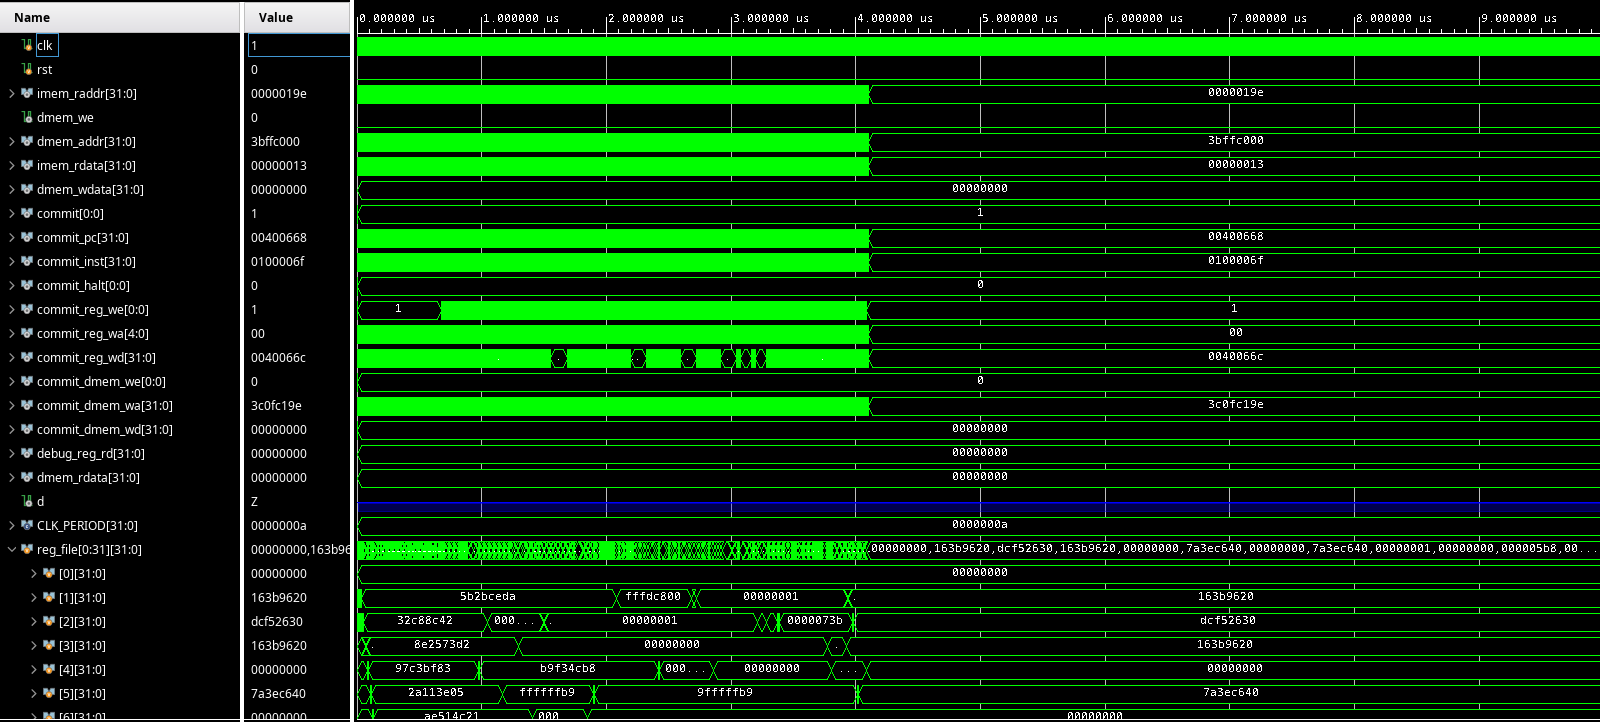
\includegraphics[scale=0.35]{pic/3.png}
    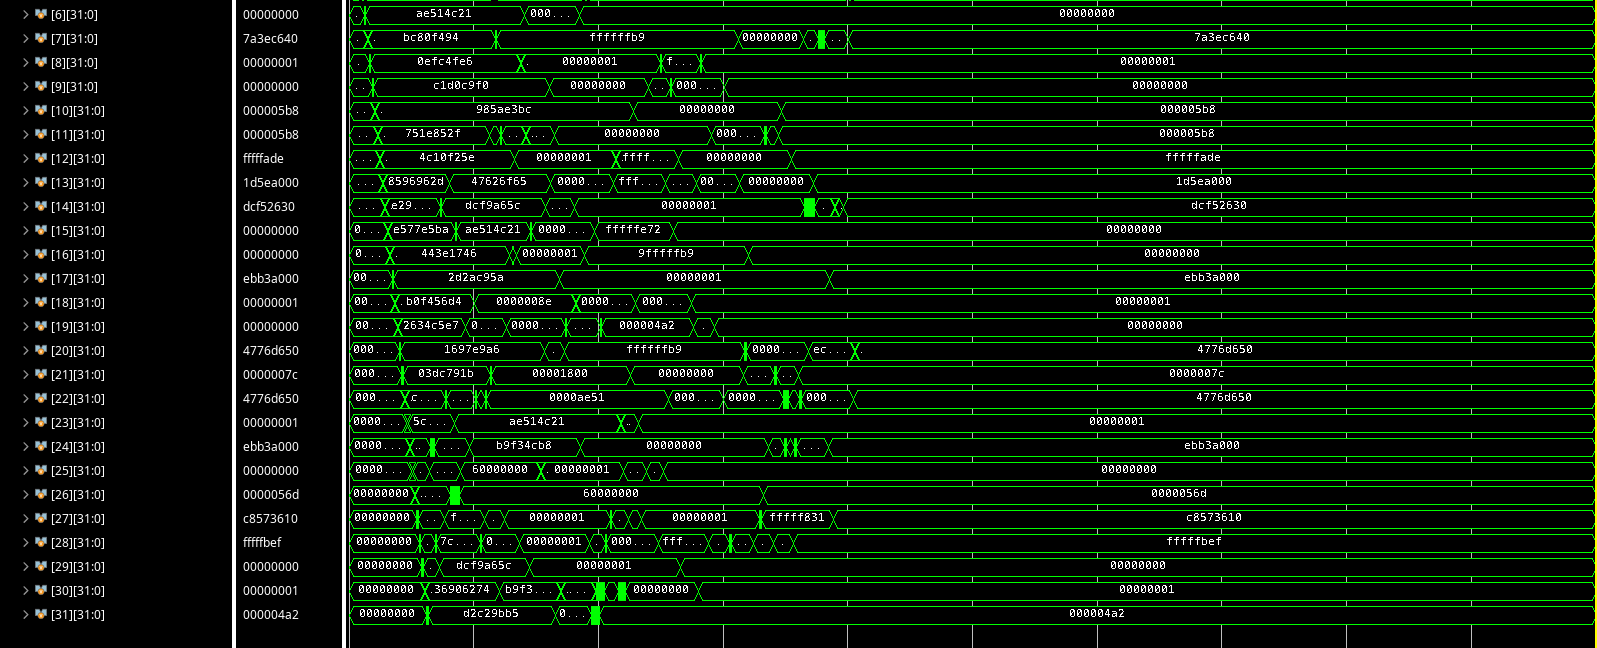
\includegraphics[scale=0.35]{pic/4.png}
    \caption{test1(普通测试)仿真结果}
\end{figure}
\begin{figure}[H]
    \centering
    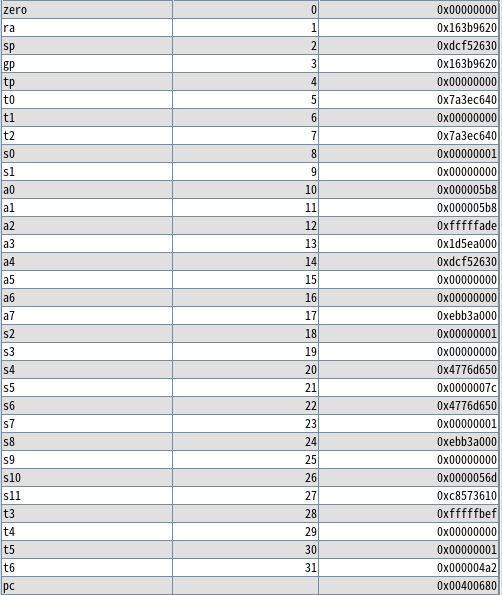
\includegraphics[scale=1]{pic/5.png}
    \caption{真实结果}
\end{figure}
仿真结果与真实结果相对应。
\subsection{test2(分支与访存测试)}
\begin{figure}[H]
    \centering
    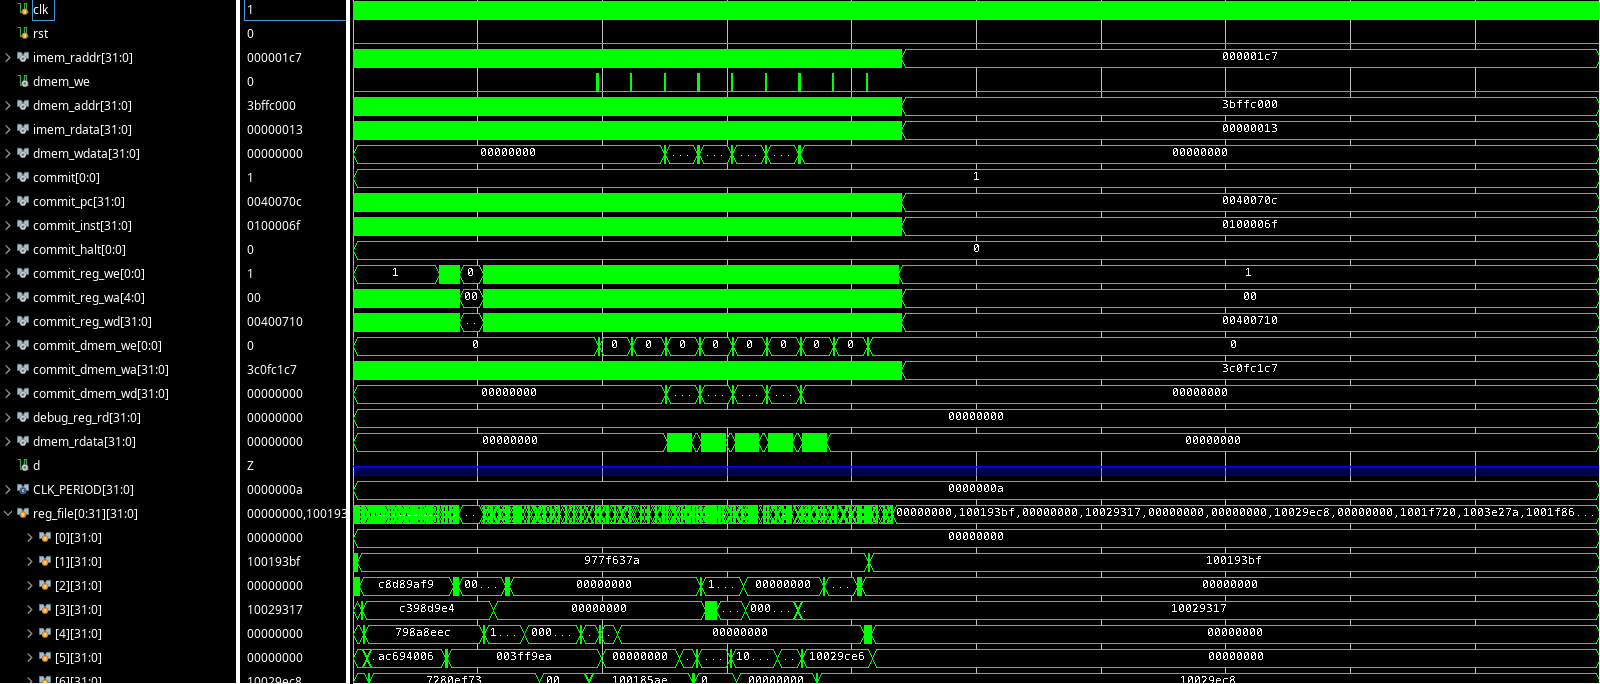
\includegraphics[scale=0.35]{pic/6.png}
    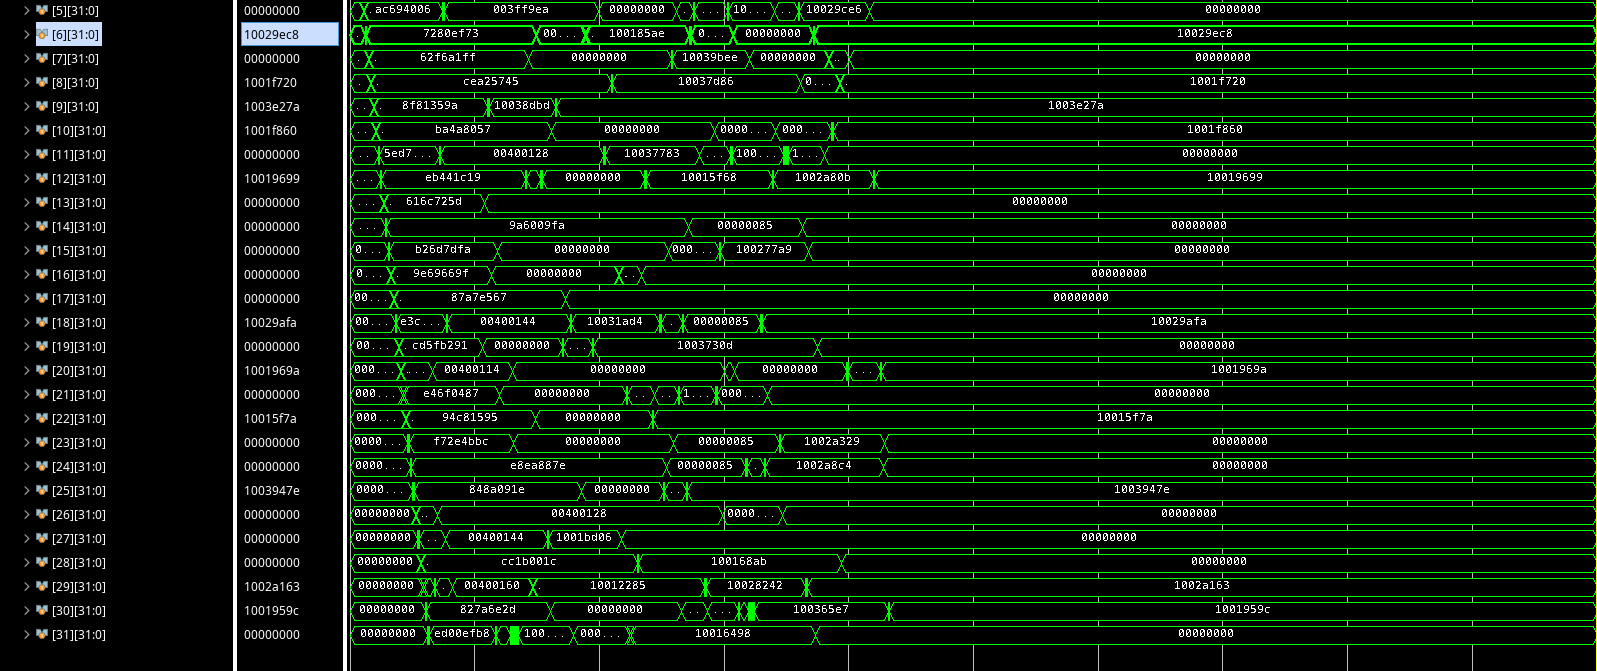
\includegraphics[scale=0.35]{pic/7.png}
    \caption{test2(分支与访存测试)}
\end{figure}
\begin{figure}[H]
    \centering
    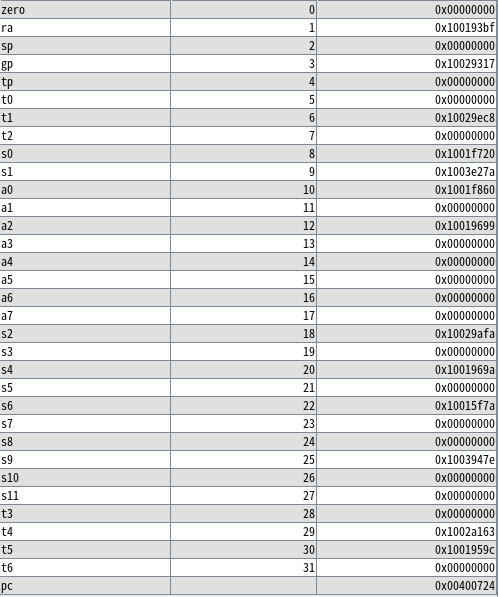
\includegraphics[scale=1]{pic/8.png}
    \caption{真实结果}
\end{figure}
仿真结果与真实结果相对应。
\subsection{斐波那契数列}
\begin{figure}[H]
    \centering
    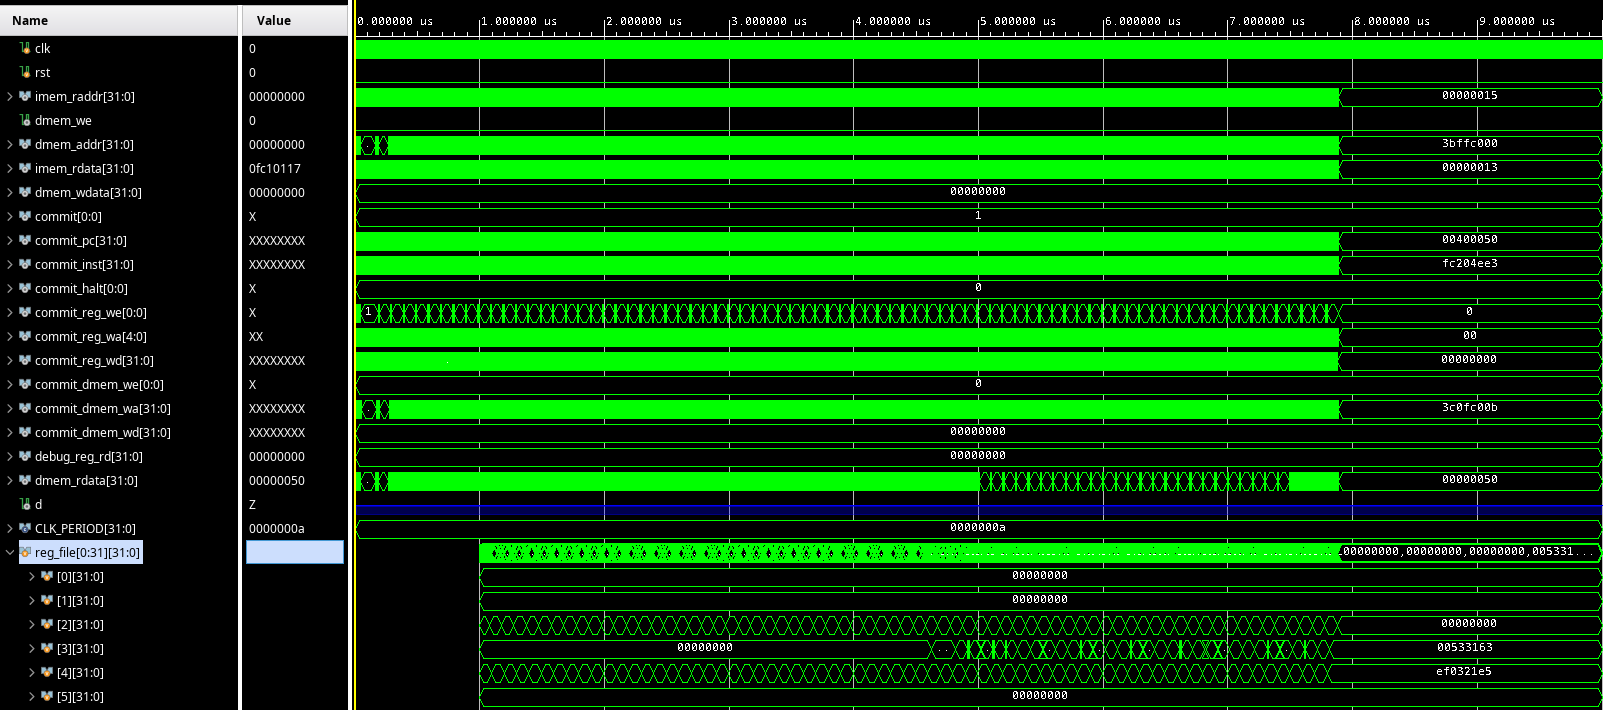
\includegraphics[scale=0.35]{pic/1.png}
    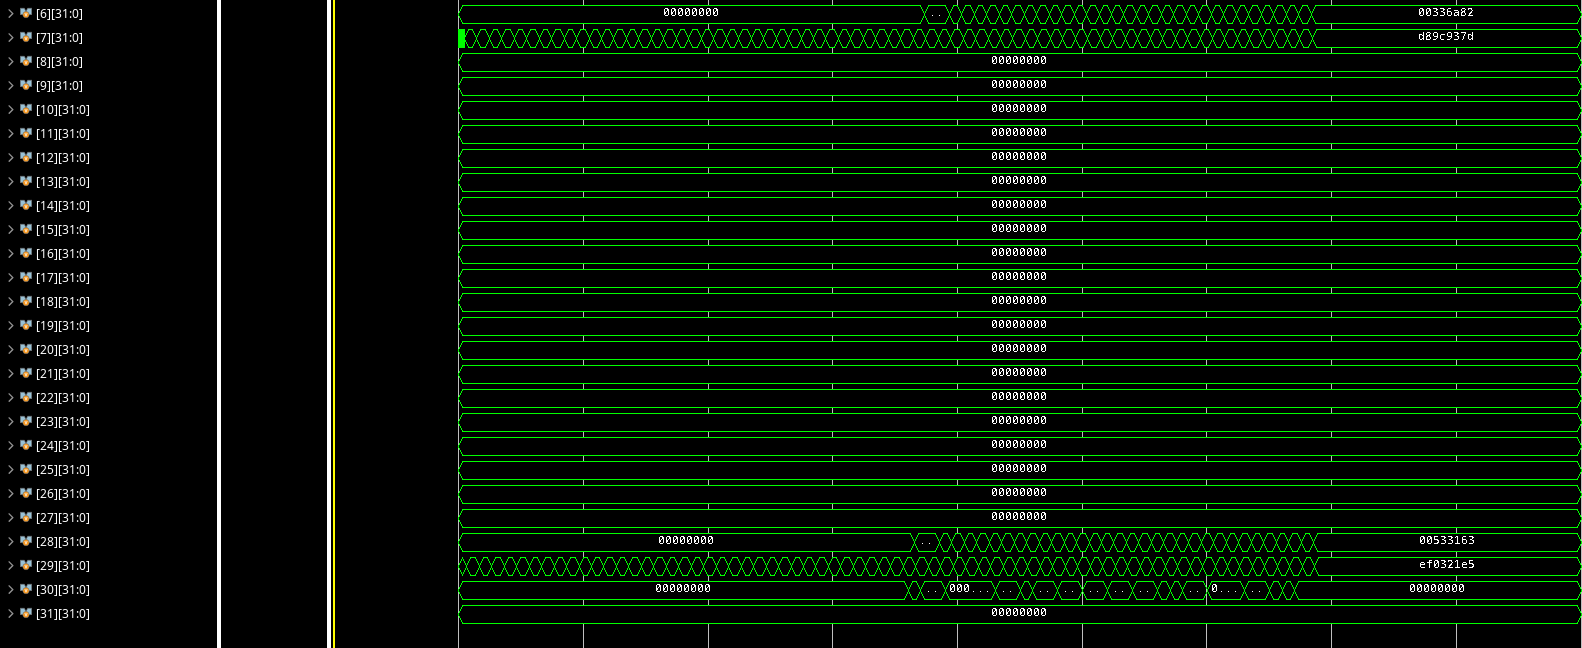
\includegraphics[scale=0.35]{pic/2.png}
    \caption{大整数版本的斐波那契数列,输入N=80,x3和x4寄存器分别存储结果的高位与低位}
\end{figure}
仿真的出的结果为533163\underline{~}ef0321e5('H23416728348467685),与正确结果相一致。
\section{电路设计与分析}
\begin{figure}[H]
    \centering
    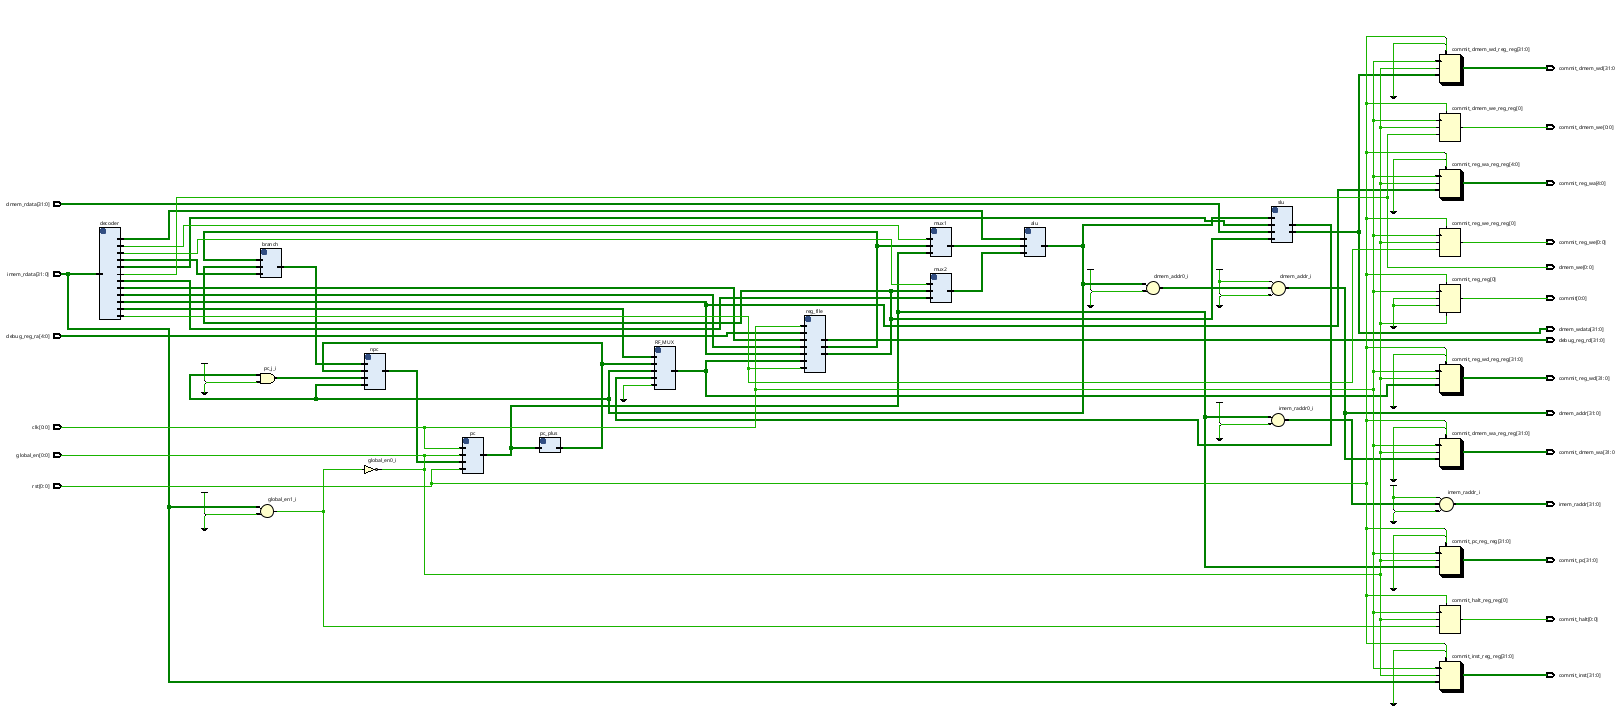
\includegraphics[scale=0.4]{pic/9.png}
    \caption{CPU}
    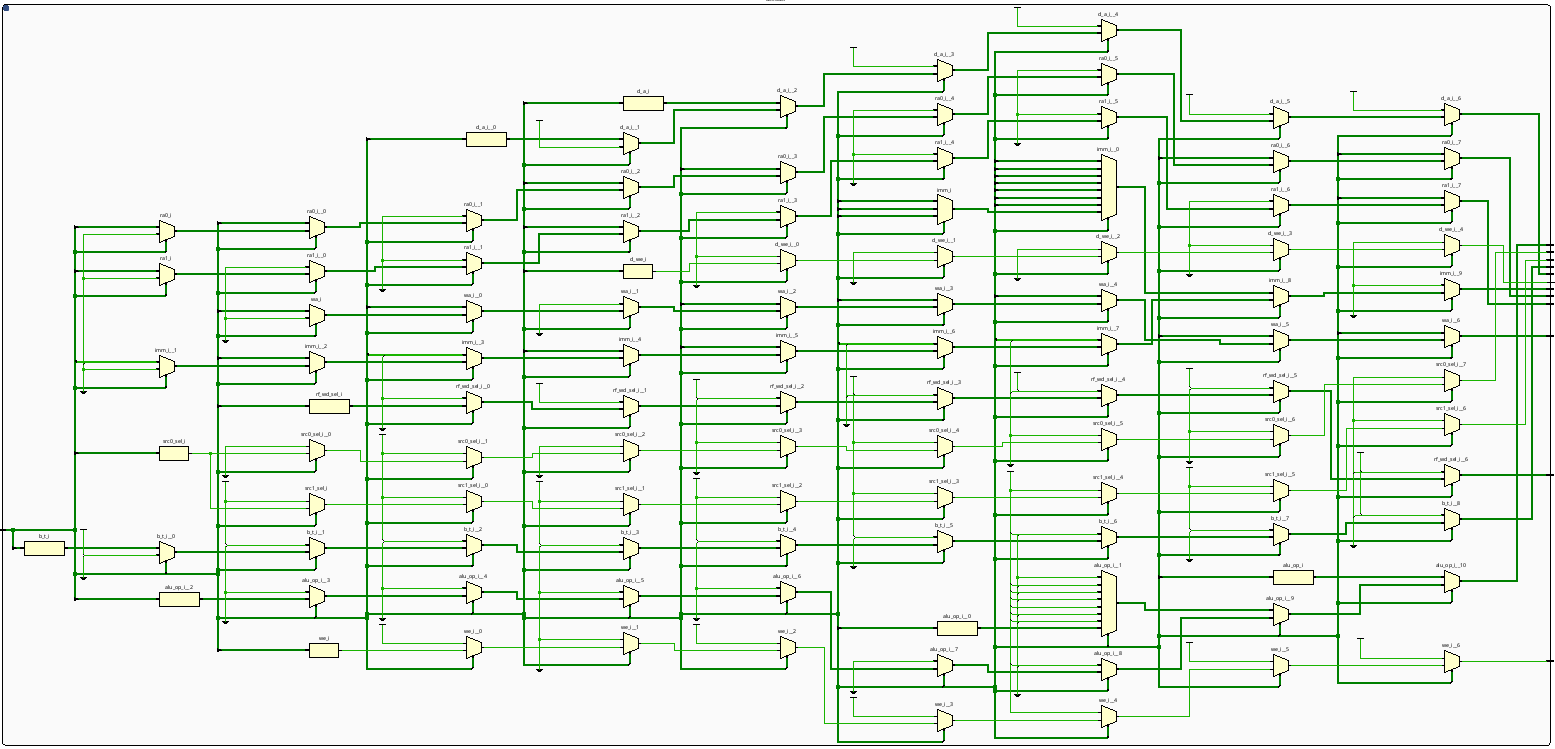
\includegraphics[scale=0.4]{pic/decoder.png}
    \caption{DECODER}
\end{figure}
\begin{figure}[H]
    \centering
    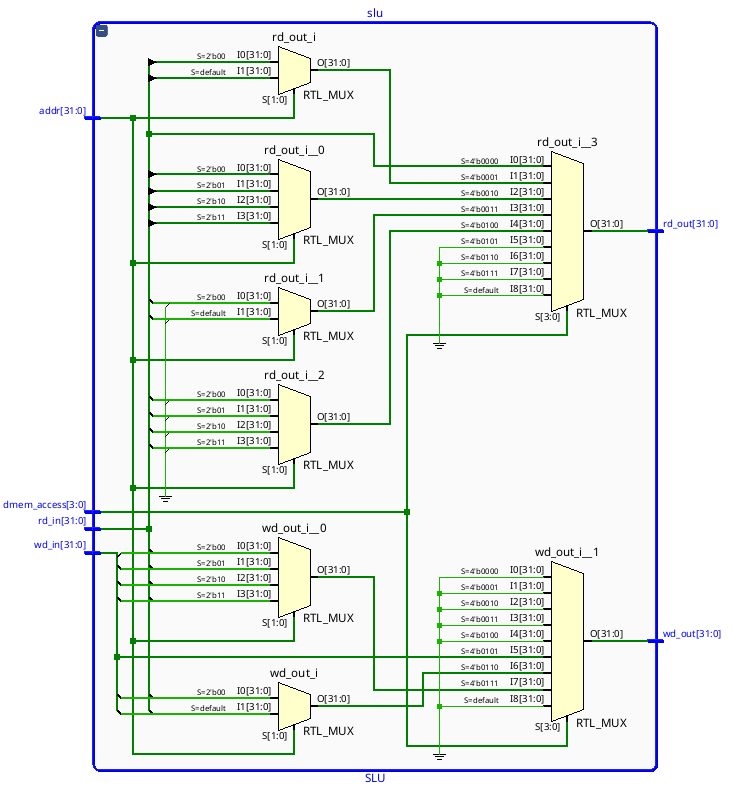
\includegraphics[scale=0.7]{pic/slu.png}
    \caption{SLU}
\end{figure}
\section{测试结果与分析}
\begin{figure}[H]
    \centering
    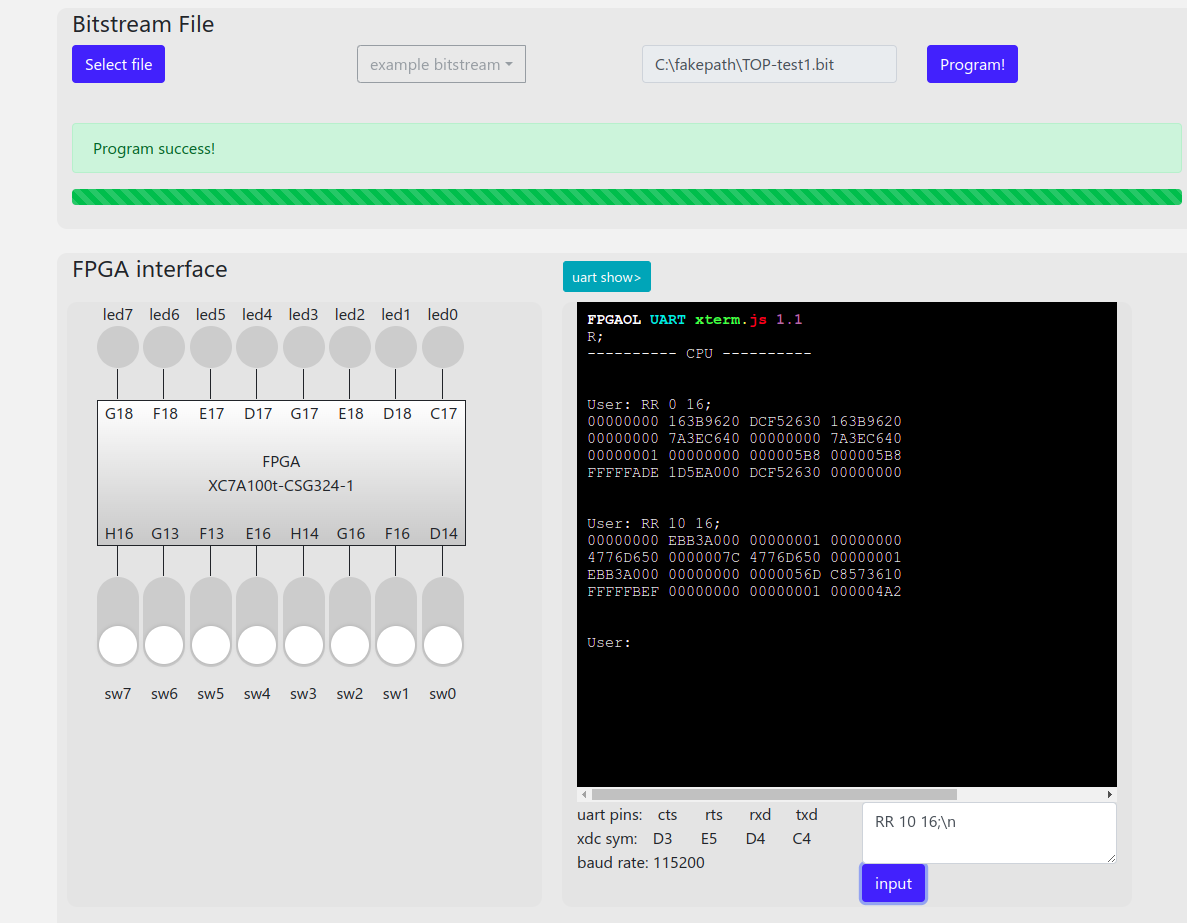
\includegraphics[scale=0.5]{pic/test1.png}
    \caption{test1(普通测试)仿真结果}
\end{figure}
\begin{figure}[H]
    \centering
    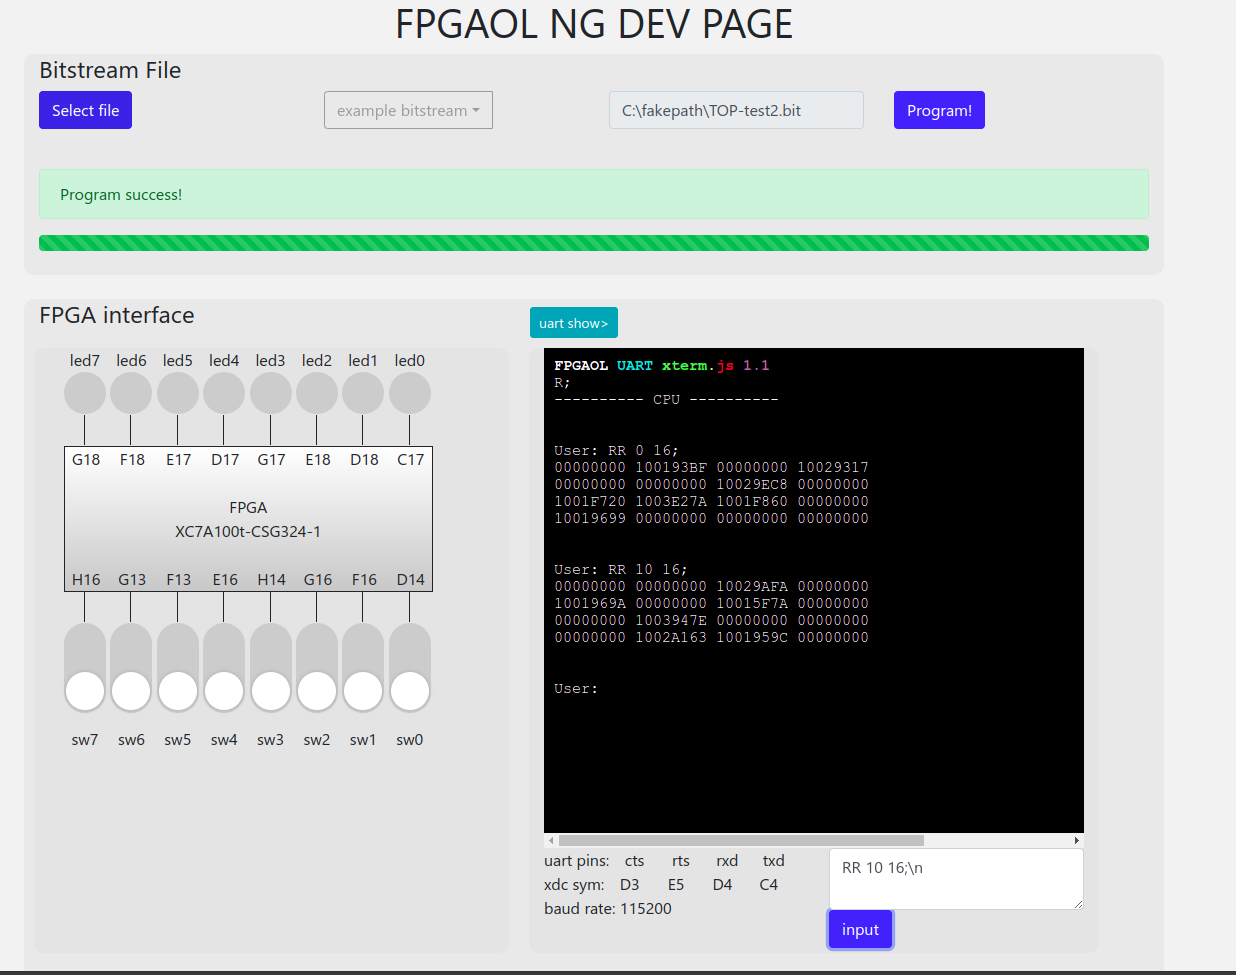
\includegraphics[scale=0.5]{pic/test2.png}
    \caption{test2(分支与访存测试)}
\end{figure}
\begin{figure}[H]
    \centering
    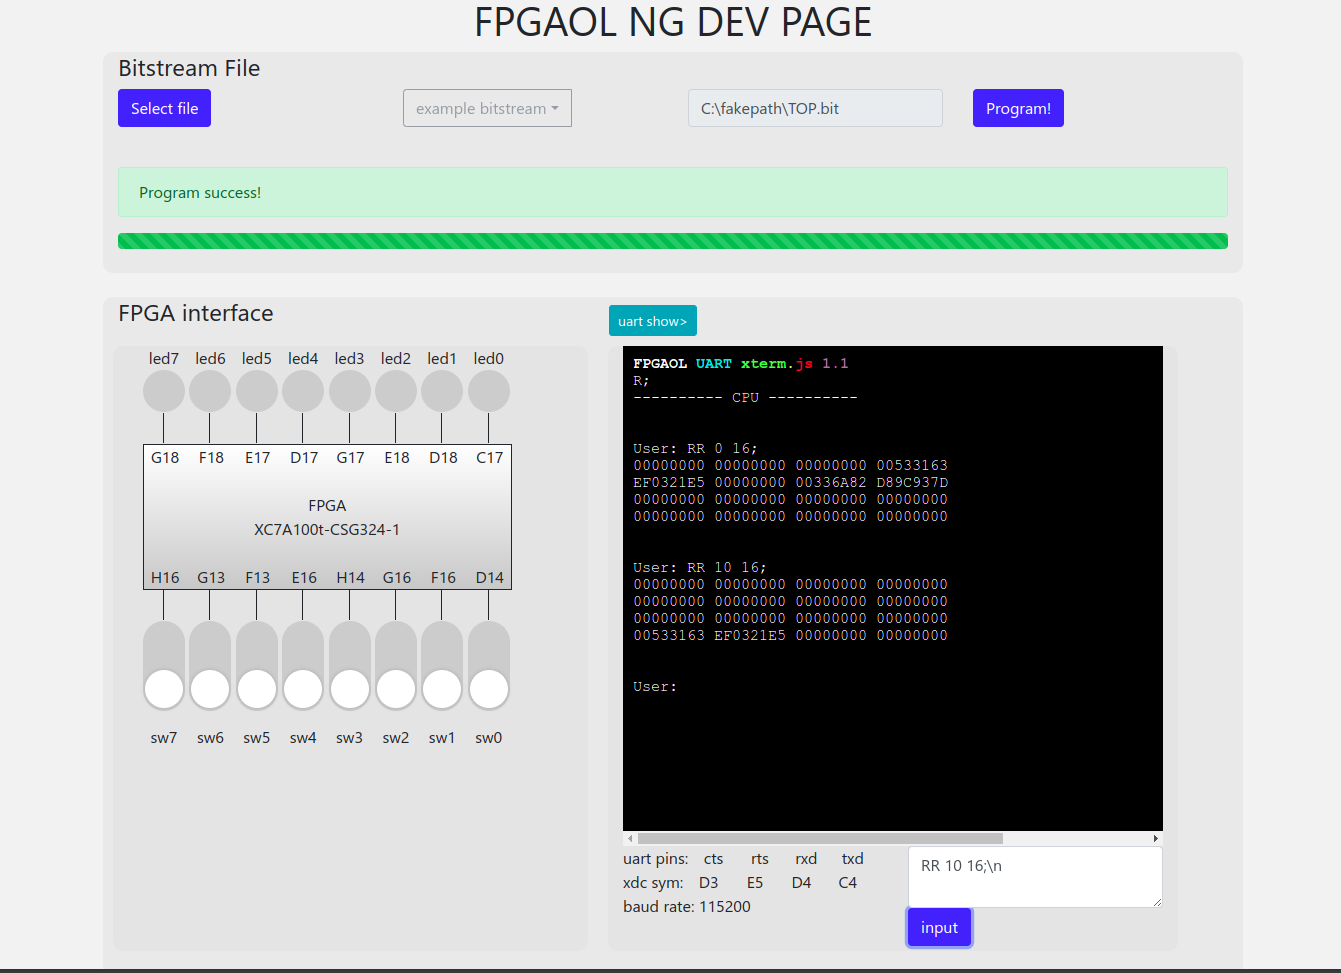
\includegraphics[scale=0.5]{pic/f.png}
    \caption{大整数版本的斐波那契数列,输入N=80,x3和x4寄存器分别存储结果的高位与低位}
\end{figure}
\section{思考与总结}
\subsection{掩码访问}
SLU代码如下:
\begin{lstlisting}[style=verilog]
`define LW 4'b0000
`define LH 4'b0001
`define LB 4'b0010
`define LHU 4'b0011
`define LBU 4'b0100
`define SW 4'b0101
`define SH 4'b0110
`define SB 4'b0111
module SL_UNIT  (input [31 : 0] addr,
            input [3 : 0] dmem_access,
            input [31 : 0] rd_in,
            input [31 : 0] wd_in,
            output reg [31 : 0] rd_out,
            output reg [31 : 0] wd_out,
            output reg [0:3] mask);
wire [31:0] addr_;
initial begin
    rd_out=0;
    wd_out=0;
    mask=0;
end
assign addr_=addr-32'h10010000;
always @(*) begin
    case(dmem_access)
        `LW:
        begin
            mask=4'b1111;
            rd_out = rd_in;
            wd_out =0;
        end
        `LH:begin
            mask=4'b1111;
            wd_out =0;
            if(addr_%4 == 0)
                rd_out = {{16{rd_in[15]}},rd_in[15:0]};
            else
                rd_out = {{16{rd_in[31]}},rd_in[31:16]};
        end
        `LB:begin
            mask=4'b1111;
            case(addr_%4)
                0:rd_out = {{24{rd_in[7]}},rd_in[7:0]};
                1:rd_out = {{24{rd_in[15]}},rd_in[15:8]};
                2:rd_out = {{24{rd_in[23]}},rd_in[23:16]};
                3:rd_out = {{24{rd_in[31]}},rd_in[31:24]};
            endcase
            wd_out =0;
        end
            
        `LHU:begin
            mask=4'b1111;
            if(addr_%4 == 0)
                rd_out = {16'b0,rd_in[15:0]};
            else
                rd_out = {16'b0,rd_in[31:16]};
            wd_out =0;
        end
            
        `LBU:begin
            mask=4'b1111;
            case(addr_%4)
                0:rd_out = {24'b0,rd_in[7:0]};
                1:rd_out = {24'b0,rd_in[15:8]};
                2:rd_out = {24'b0,rd_in[23:16]};
                3:rd_out = {24'b0,rd_in[31:24]};
            endcase
            wd_out =0;
        end
        `SW:begin
            mask=4'b1111;
            wd_out=wd_in;
            rd_out = 0;
        end 
        `SH:begin
            if(addr_%4 == 0)
                mask=4'b0011;
            else
                mask=4'b1100;
            wd_out=wd_in;
            rd_out = 0;
        end
            
        `SB:begin
            case(addr_%4)
                0:mask=4'b0001;
                1:mask=4'b0010;
                2:mask=4'b0100;
                3:mask=4'b1000;
            endcase
            wd_out=wd_in;
            rd_out = 0;
        end
        default:
            begin
                mask=4'b0000;
                rd_out = 0;
                wd_out =0;
            end
    endcase
end
endmodule
\end{lstlisting}\par
在读取阶段,掩码mask统一为4'b1111,这是因为
即使利用掩码只读取所需的部分,实际返回值仍然是一个32bit的数字,
需要从中提取出有效部分,因此在我看来,在此阶段无需做额外的处理。\par
但是在写入阶段,通过掩码可以直接将一整个wd\underline{~}in写入,而无需担心
影响其他位,可以使代码更加简化。
\subsection{可能的关键路径}
\begin{figure}[H]
    \centering
    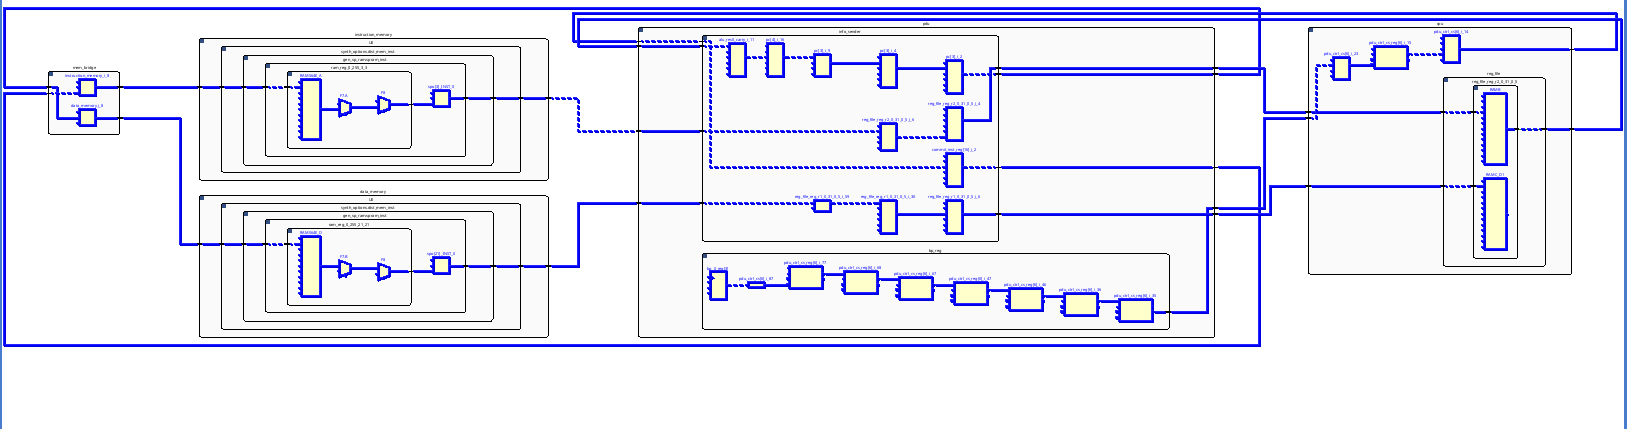
\includegraphics[scale=0.35]{pic/key.png}
    \caption{可能的关键路径}
\end{figure}
以下是对各部分放大(从左往右):
\begin{figure}[H]
    \centering
    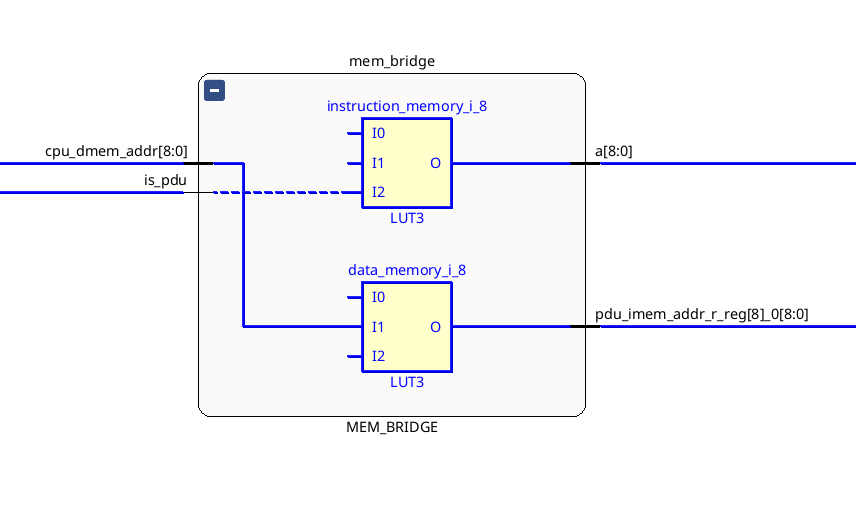
\includegraphics[scale=0.5]{pic/10.png}
    \caption{mem\underline{~}bridge}
\end{figure}
\begin{figure}[H]
    \centering
    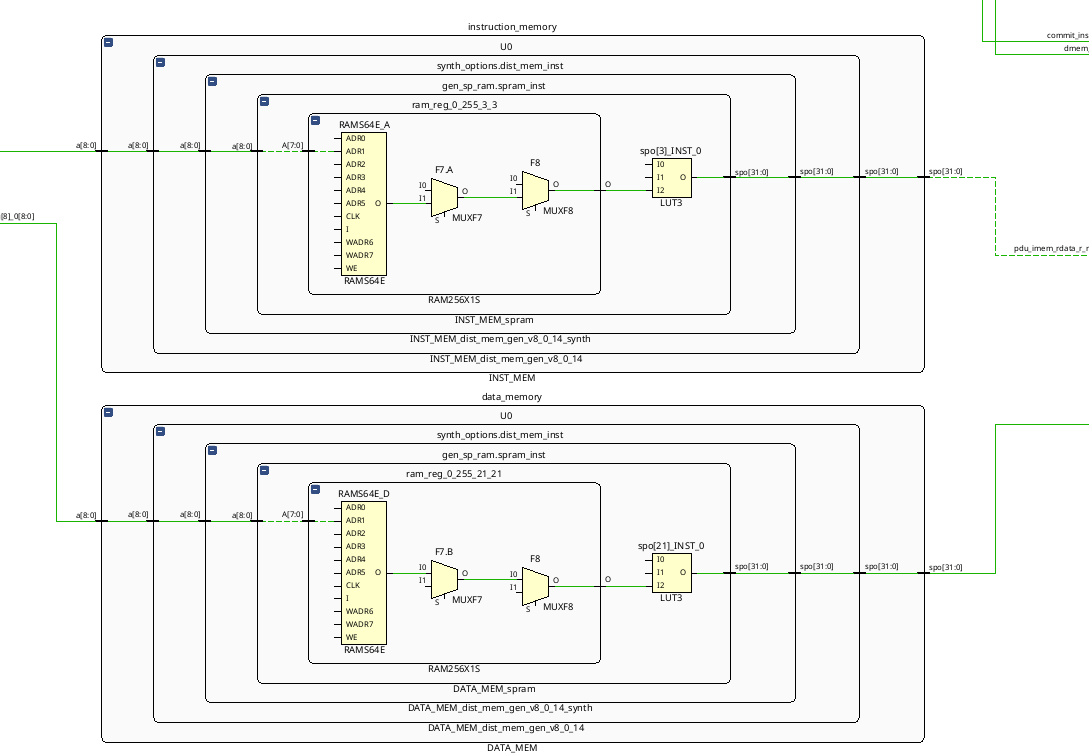
\includegraphics[scale=0.5]{pic/11.png}
    \caption{INST\underline{~}MEM和DATA\underline{~}MEM}
\end{figure}
\begin{figure}[H]
    \centering
    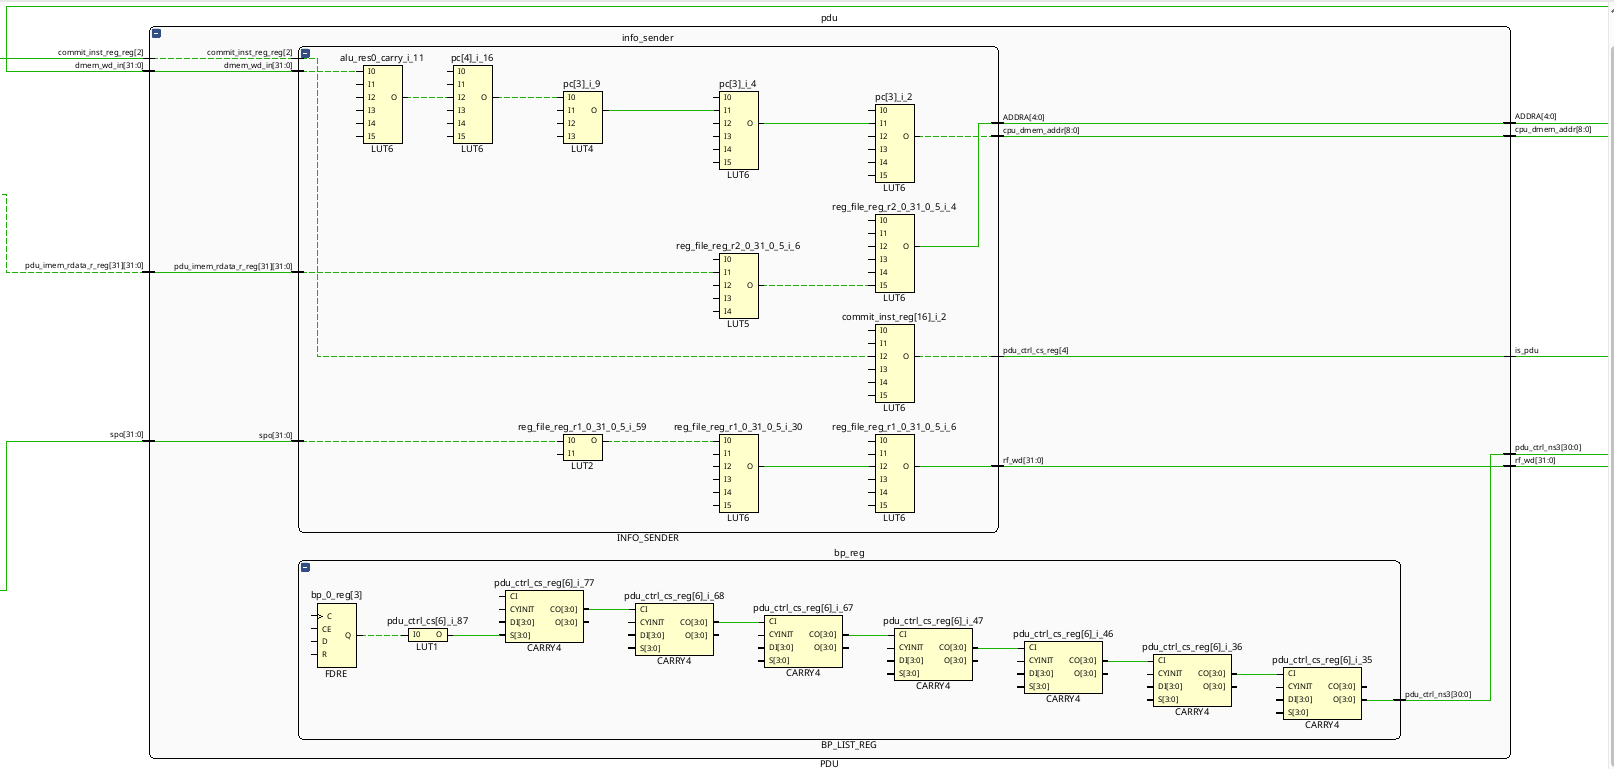
\includegraphics[scale=0.3]{pic/12.png}
    \caption{PDU}
\end{figure}
\begin{figure}[H]
    \centering
    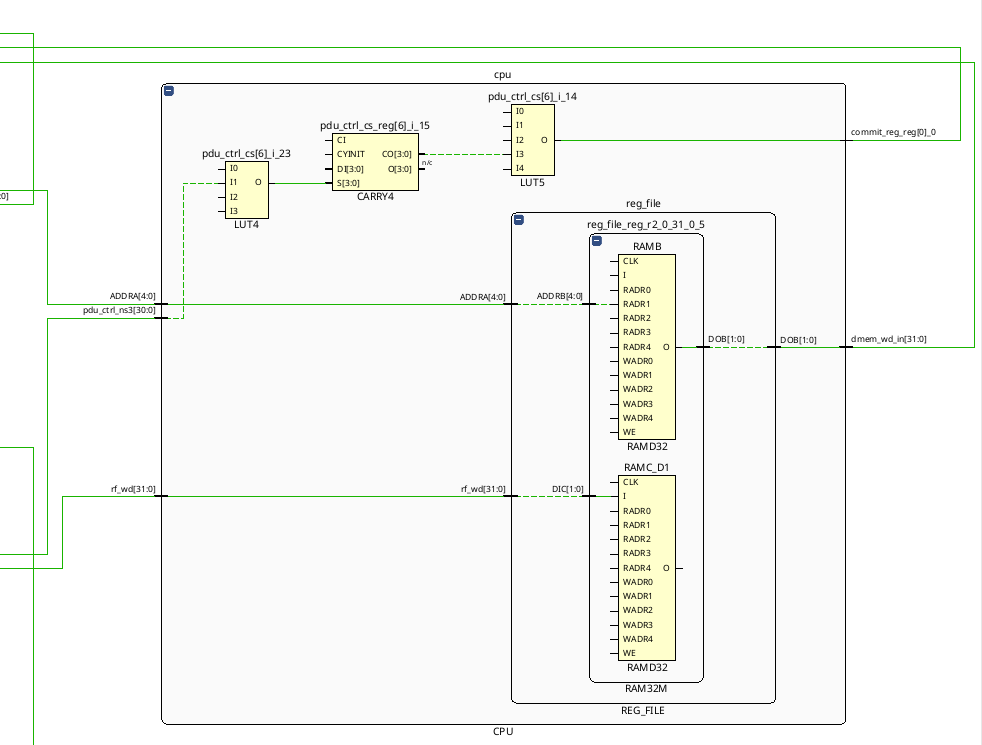
\includegraphics[scale=0.5]{pic/13.png}
    \caption{CPU}
\end{figure}
\end{document}